\section{Sequence Diagrams}

After completing the class diagrams and activity diagrams of the system, we will  demonstrate how the system's classes interact with each other according to the system's business flow using sequence diagrams.

\subsection{Self-register}

\begin{figure}[H]
    \centering
    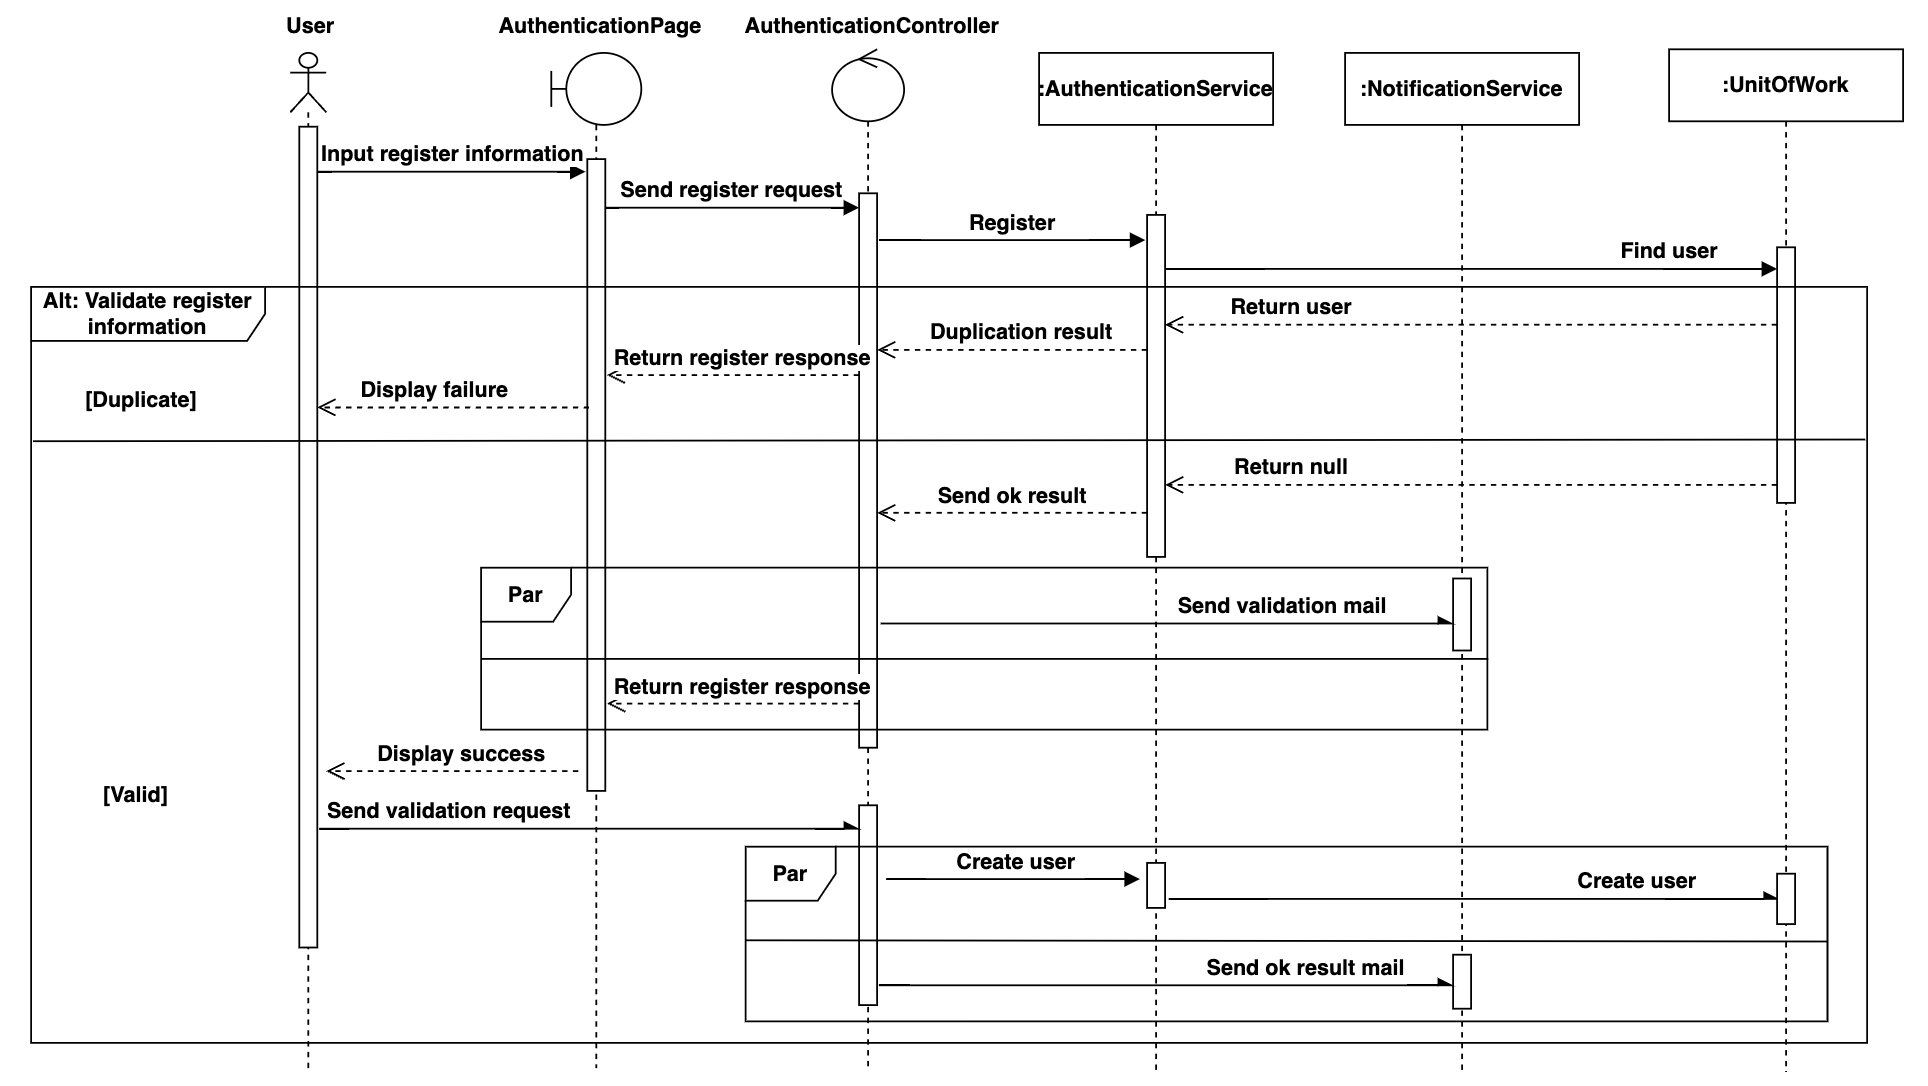
\includegraphics[width=0.85\textwidth]{Figures/self_register_seq.png}
    \caption{Self-register sequence diagram}
    \label{fig:self-registration-seq}
\end{figure}

\subsection{Login}
\begin{figure}[H]
    \centering
    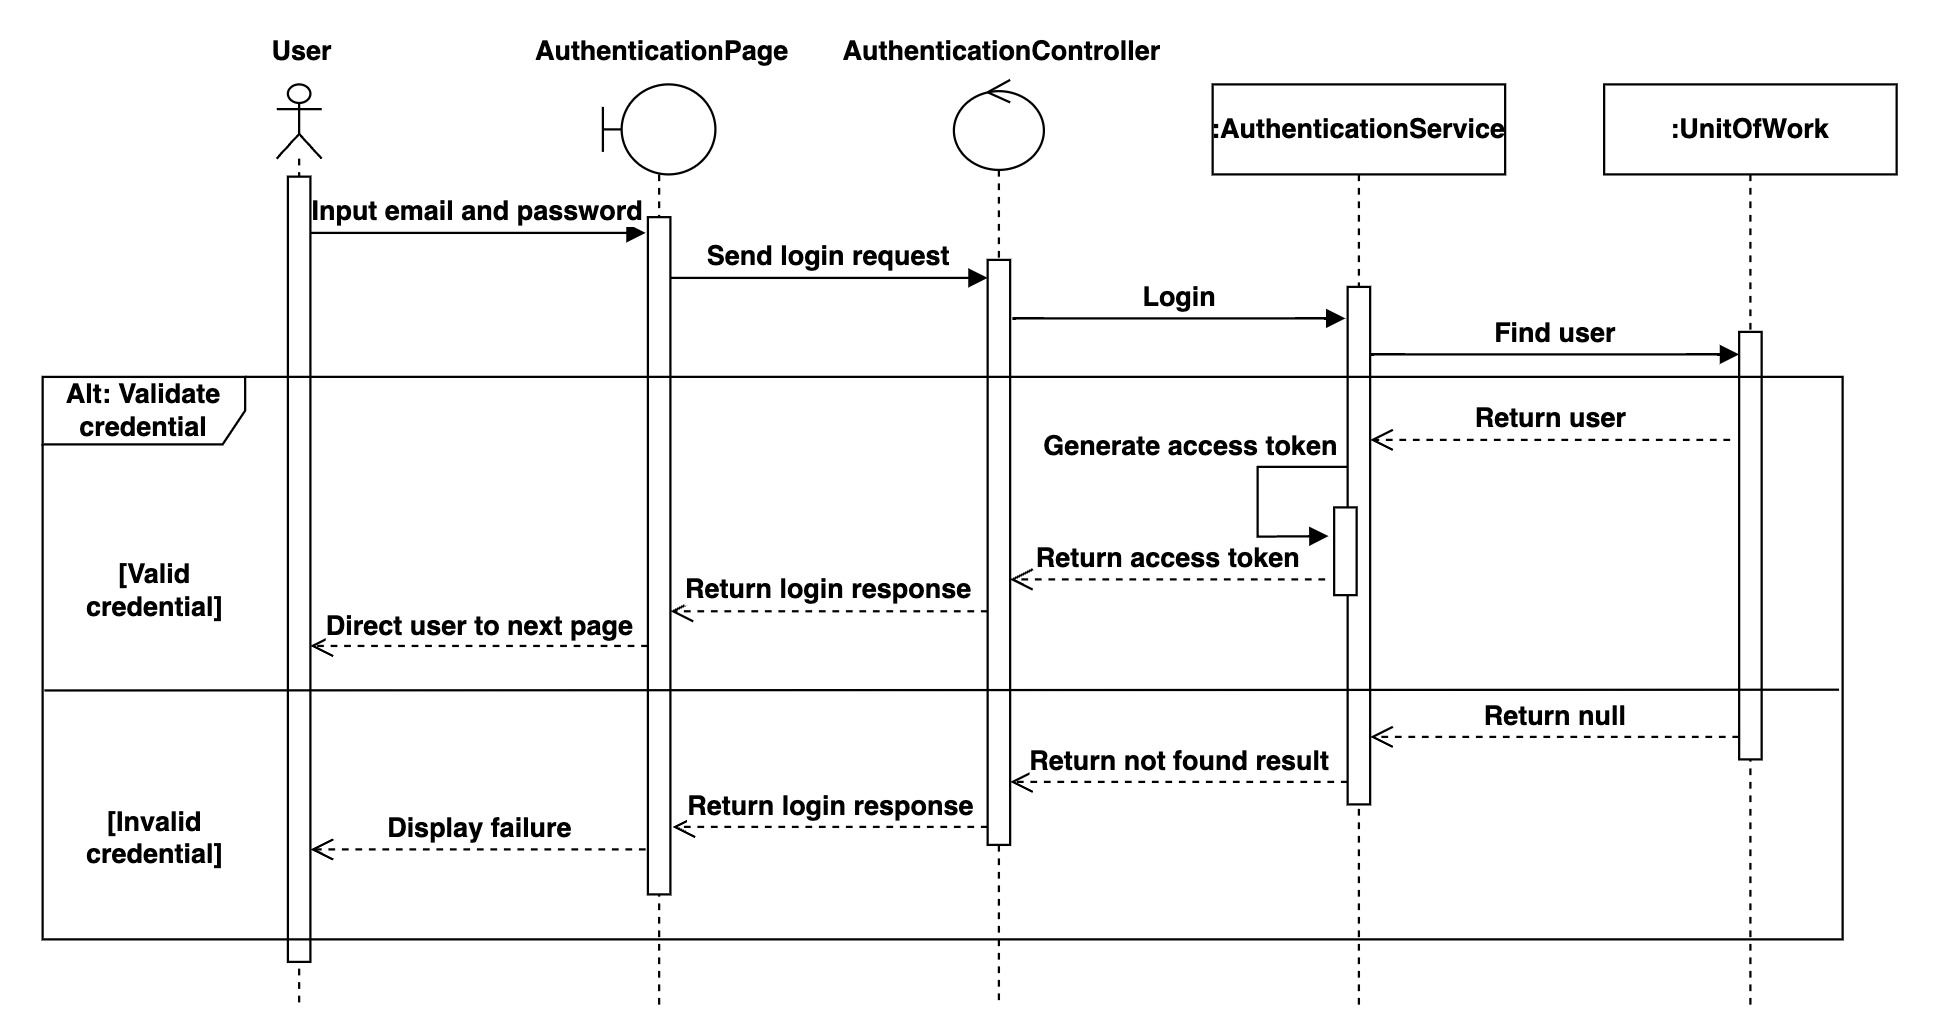
\includegraphics[width=0.85\textwidth]{Figures/login_seq.png}
    \caption{Login sequence diagram}
    \label{fig:login-seq}
\end{figure}
\subsection{Login with a Google account}

\begin{figure}[H]
    \centering
    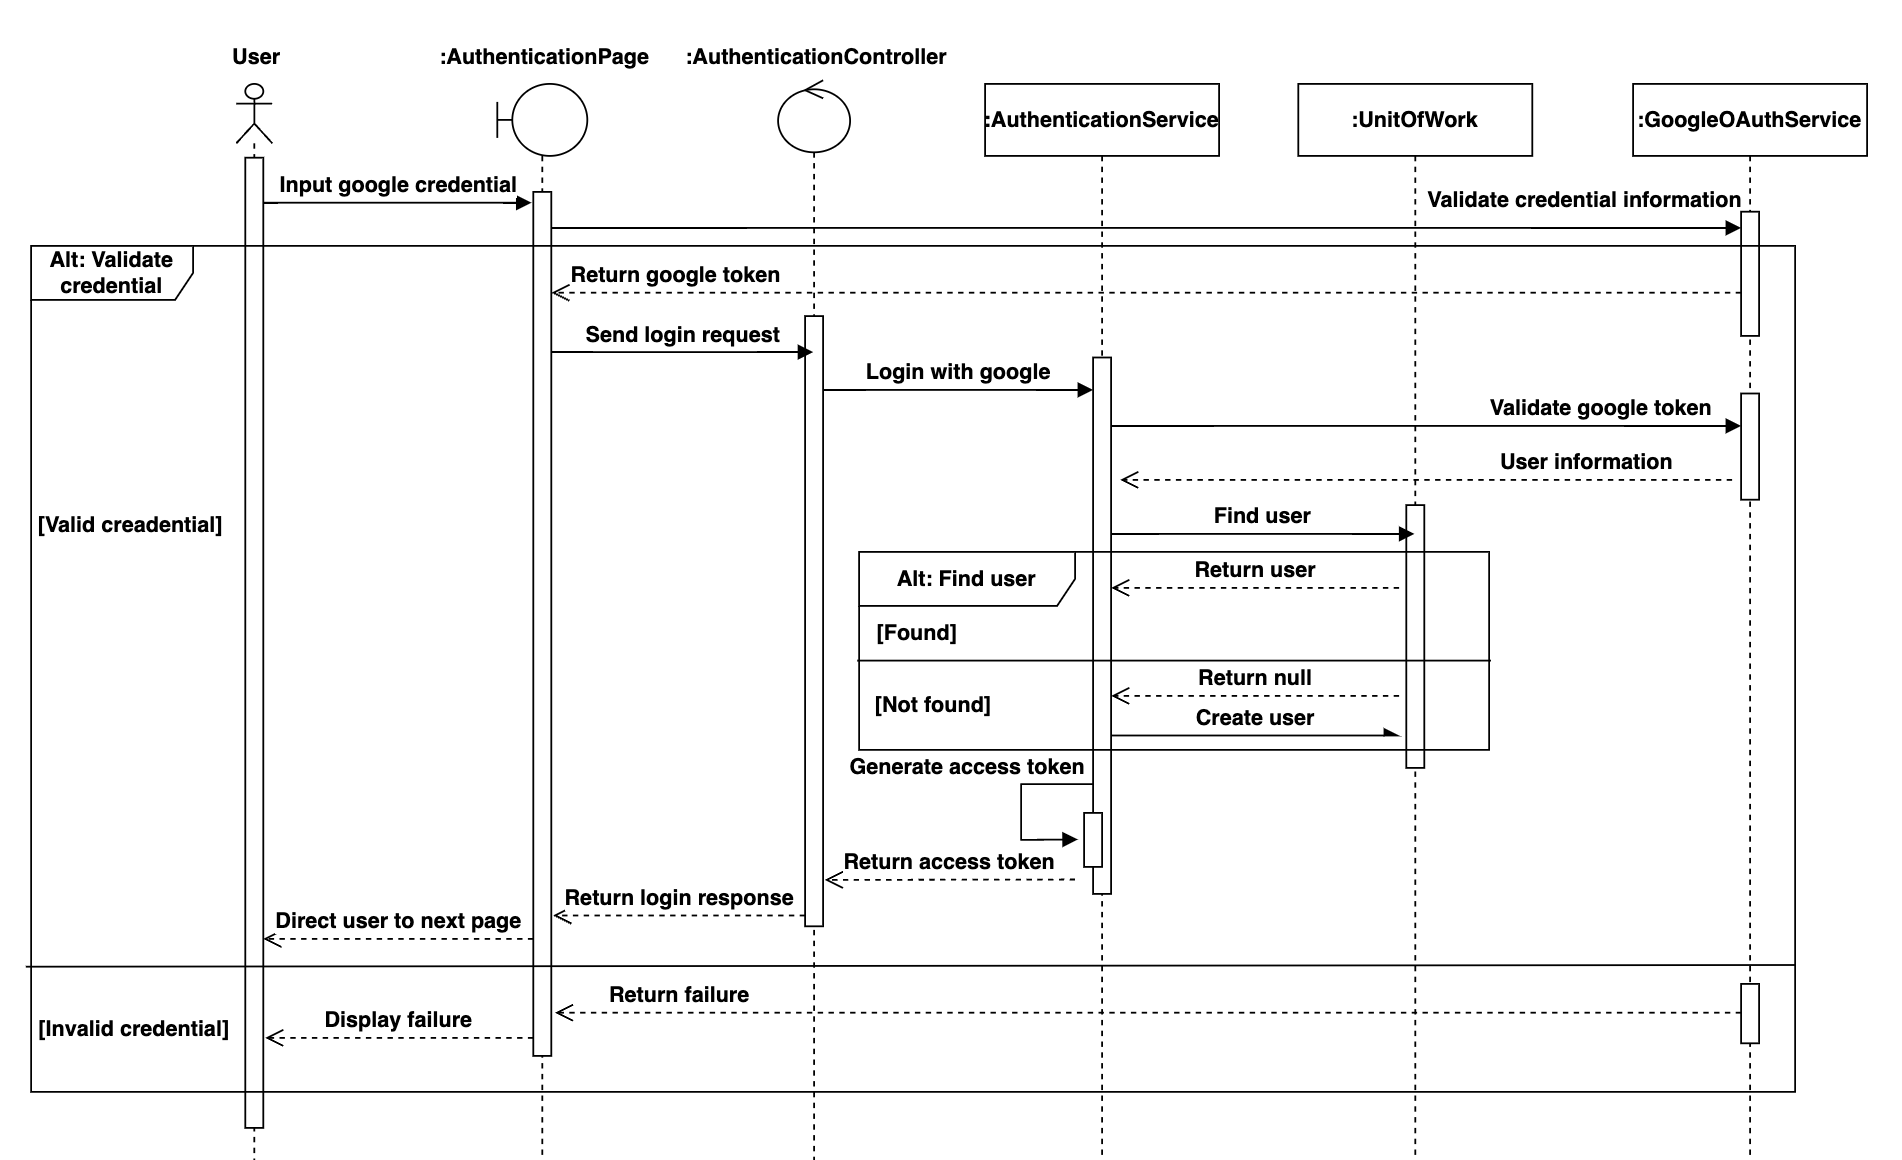
\includegraphics[width=0.9\textwidth]{Figures/login_gg_seq.png}
    \caption{Login with a Google account sequence diagram}
    \label{fig:login-google-seq}
\end{figure}

\subsection{Update to Organization account}

\begin{figure}[H]
    \centering
    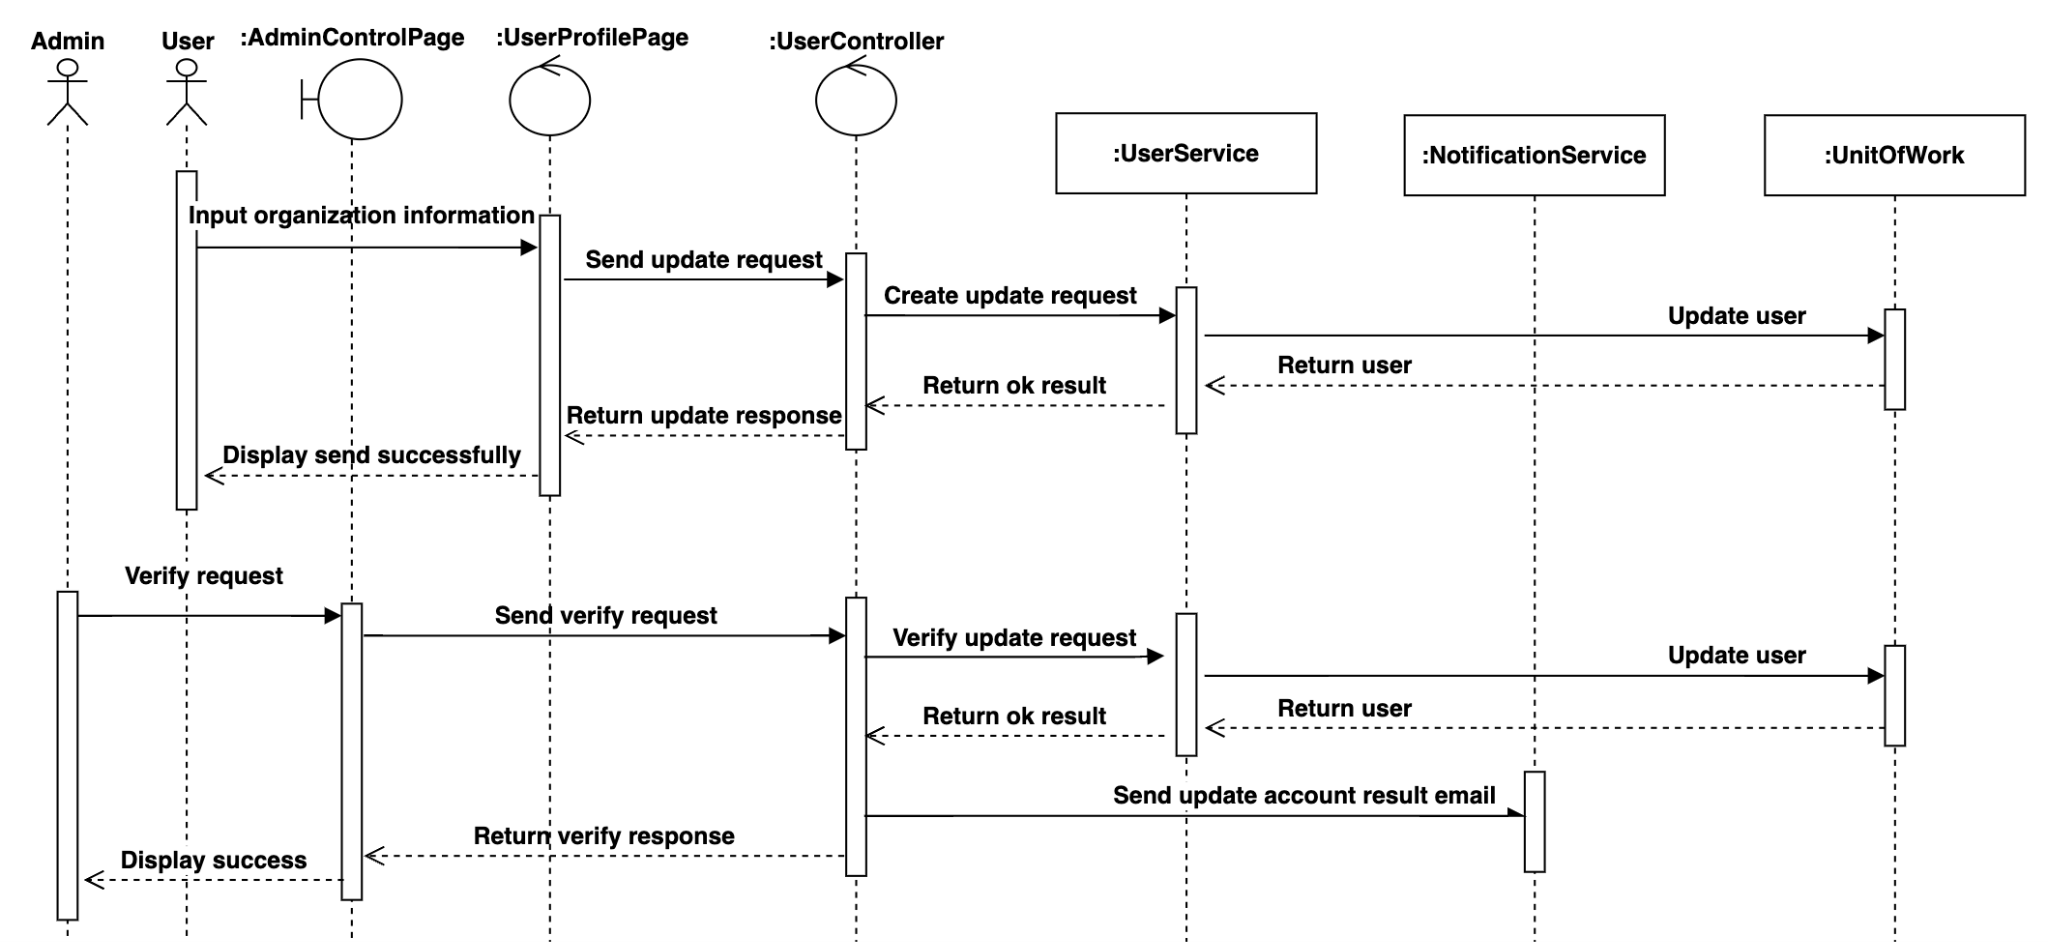
\includegraphics[width=0.9\textwidth]{Figures/update_org_seq.png}
    \caption{Update to Organization account sequence diagram}
    \label{fig:update-org-seq}
\end{figure}
\clearpage

\subsection{Manage pet profile}

\begin{figure}[H]
    \centering
    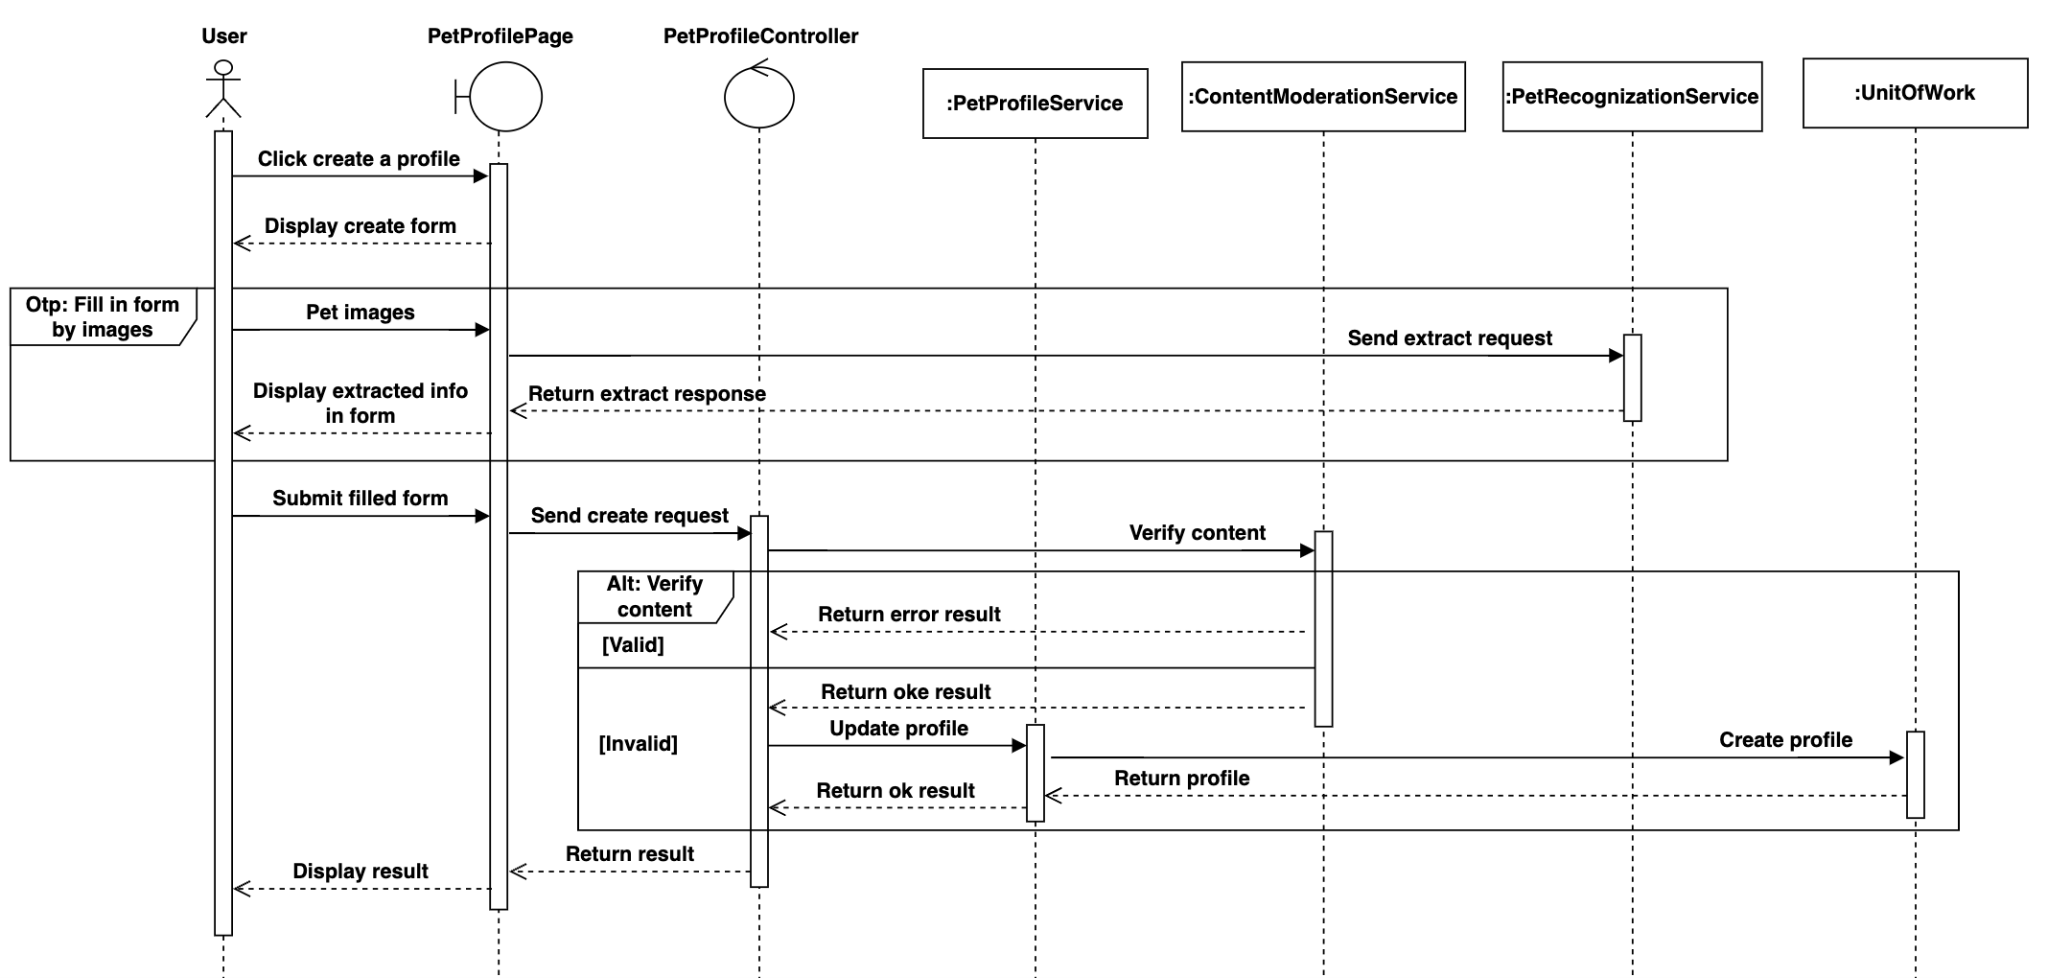
\includegraphics[angle=-90,width=0.6\textwidth]{Figures/manage_pet_seq.png}
    \caption{Manage pet profile sequence diagram}
    \label{fig:manage-pet-seq}
\end{figure}
\clearpage

\begin{figure}[H]
    \centering
    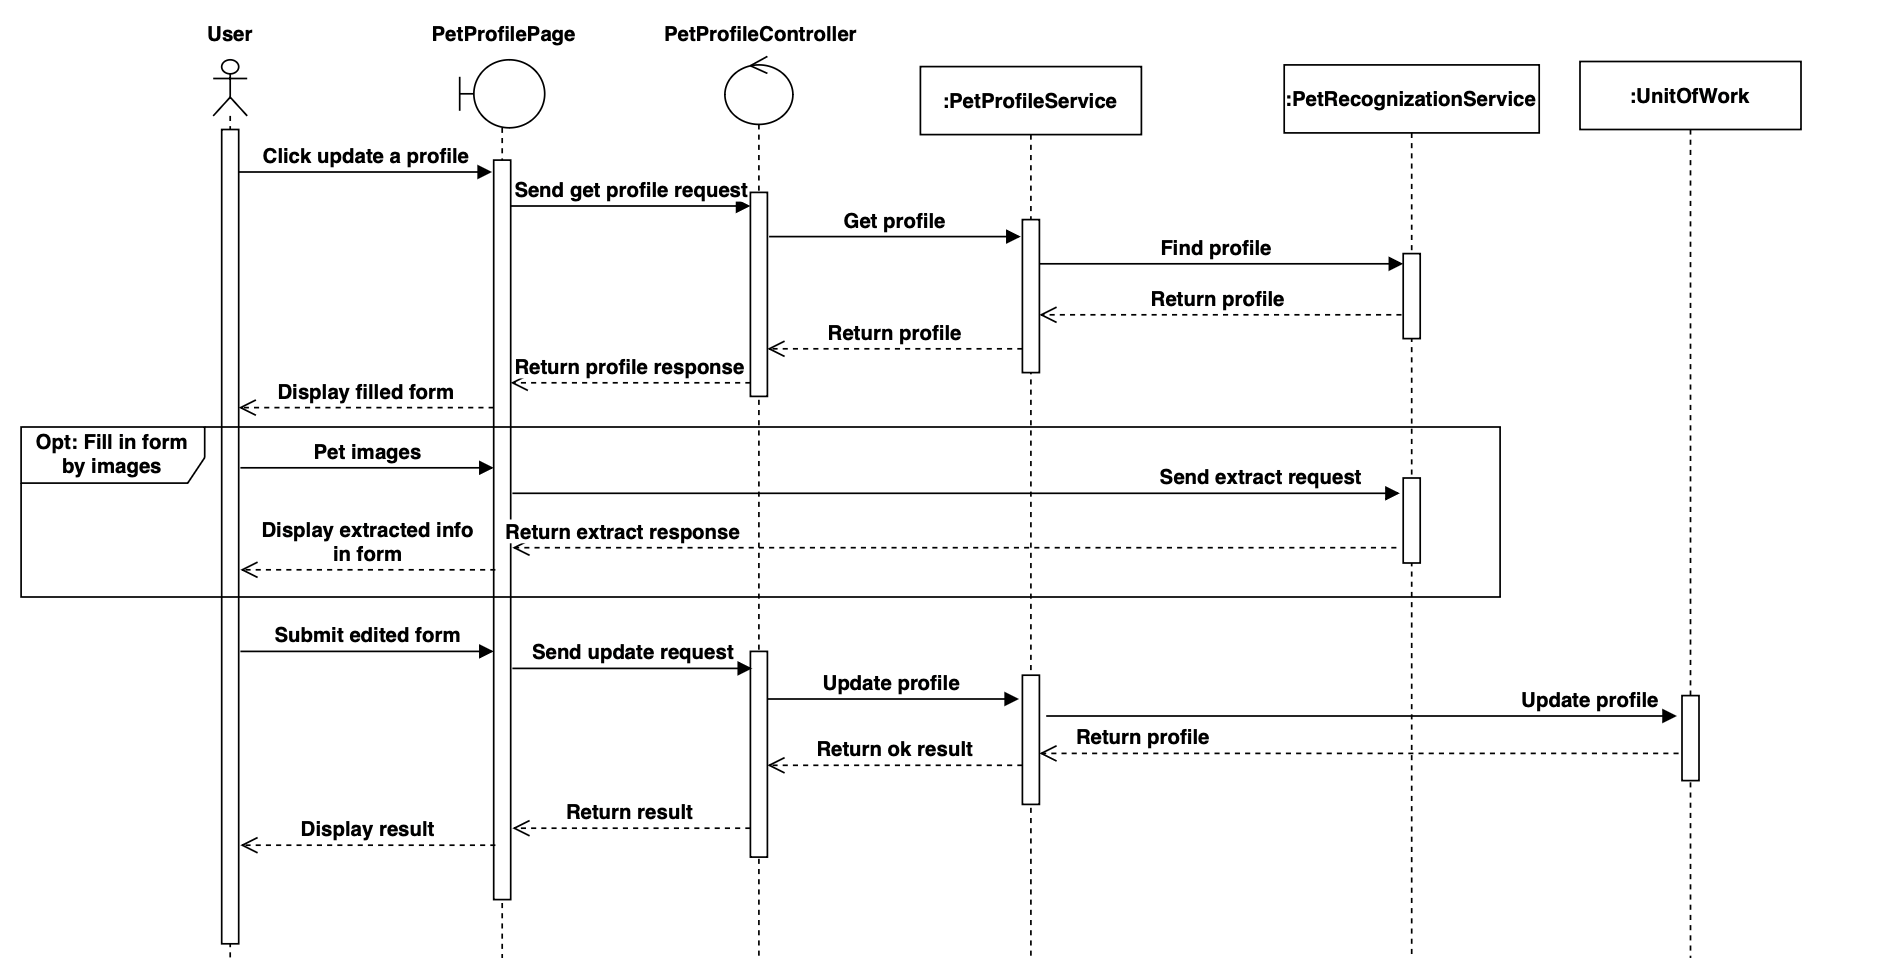
\includegraphics[angle=-90,width=0.7\textwidth]{Figures/update_pet_profile_seq.png}
    \caption{Update pet profile sequence diagram}
    \label{fig:update-pet-seq}
\end{figure}
\clearpage

\subsection{Adopt pets}
\begin{figure}[H]
    \centering
    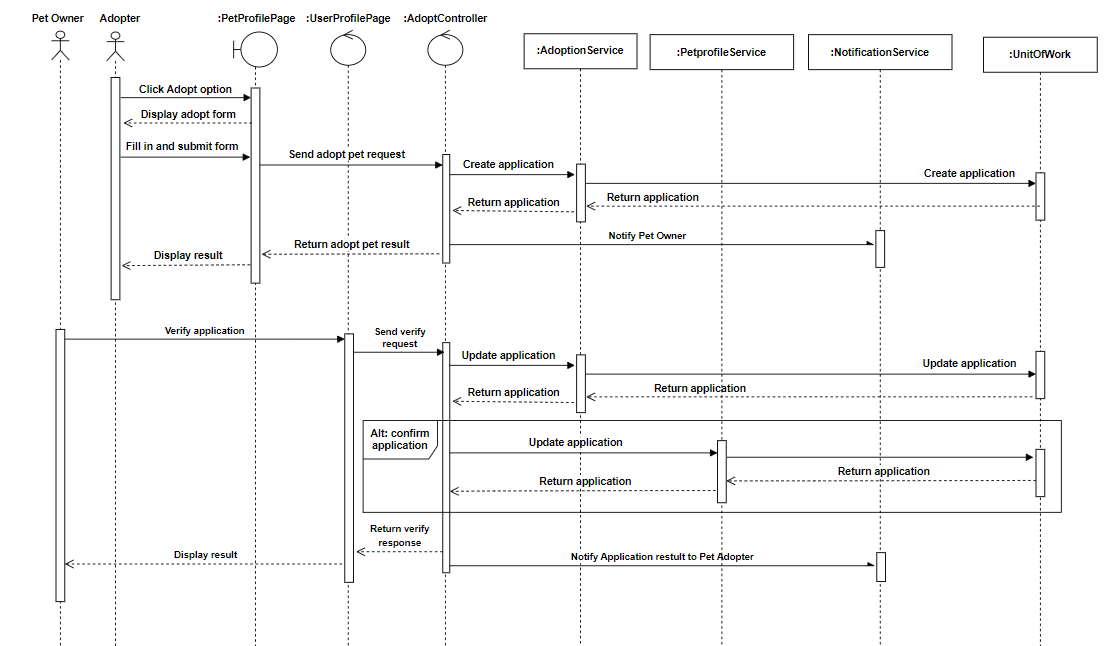
\includegraphics[angle=-90,width=0.8\textwidth]{Figures/adopt_pet_seq.png}
    \caption{Adopt pet sequence diagram}
    \label{fig:adopt-pet-seq}
\end{figure}
\clearpage

\subsection{Manage blogs}

\begin{figure}[H]
    \centering
    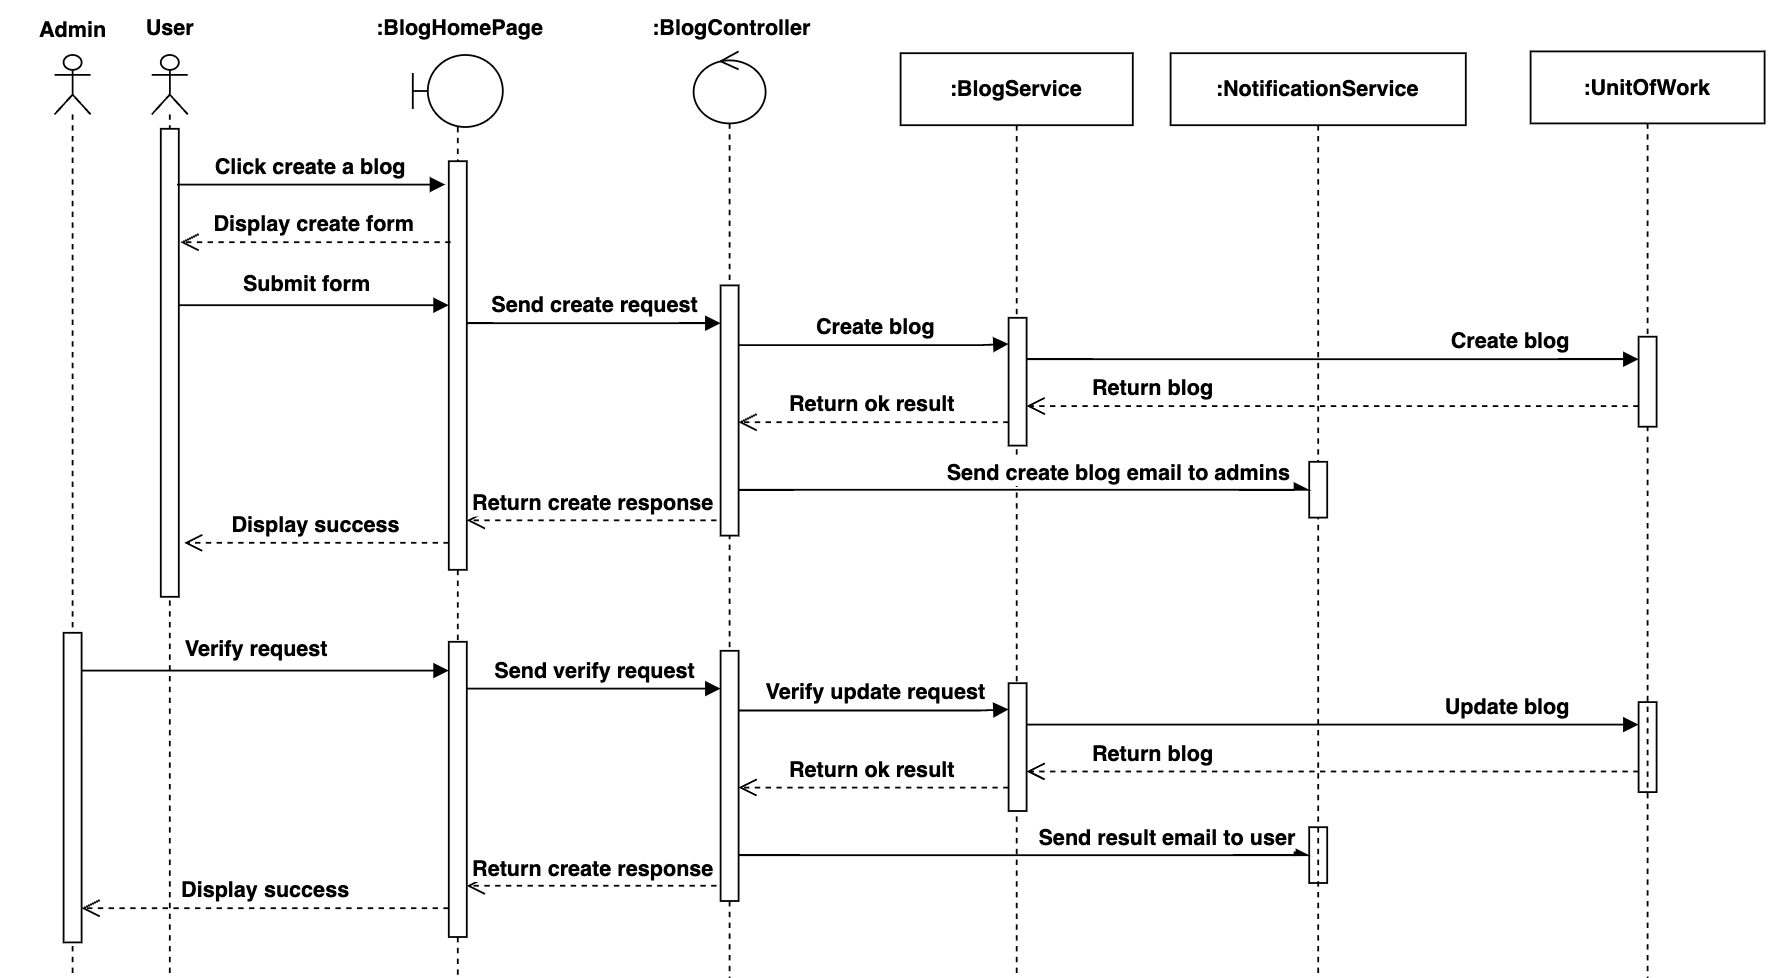
\includegraphics[width=0.9\textwidth]{Figures/manage_blog_seq.png}
    \caption{Create blogs sequence diagram}
    \label{fig:manage-blog-seq}
\end{figure}

\begin{figure}[H]
    \centering
    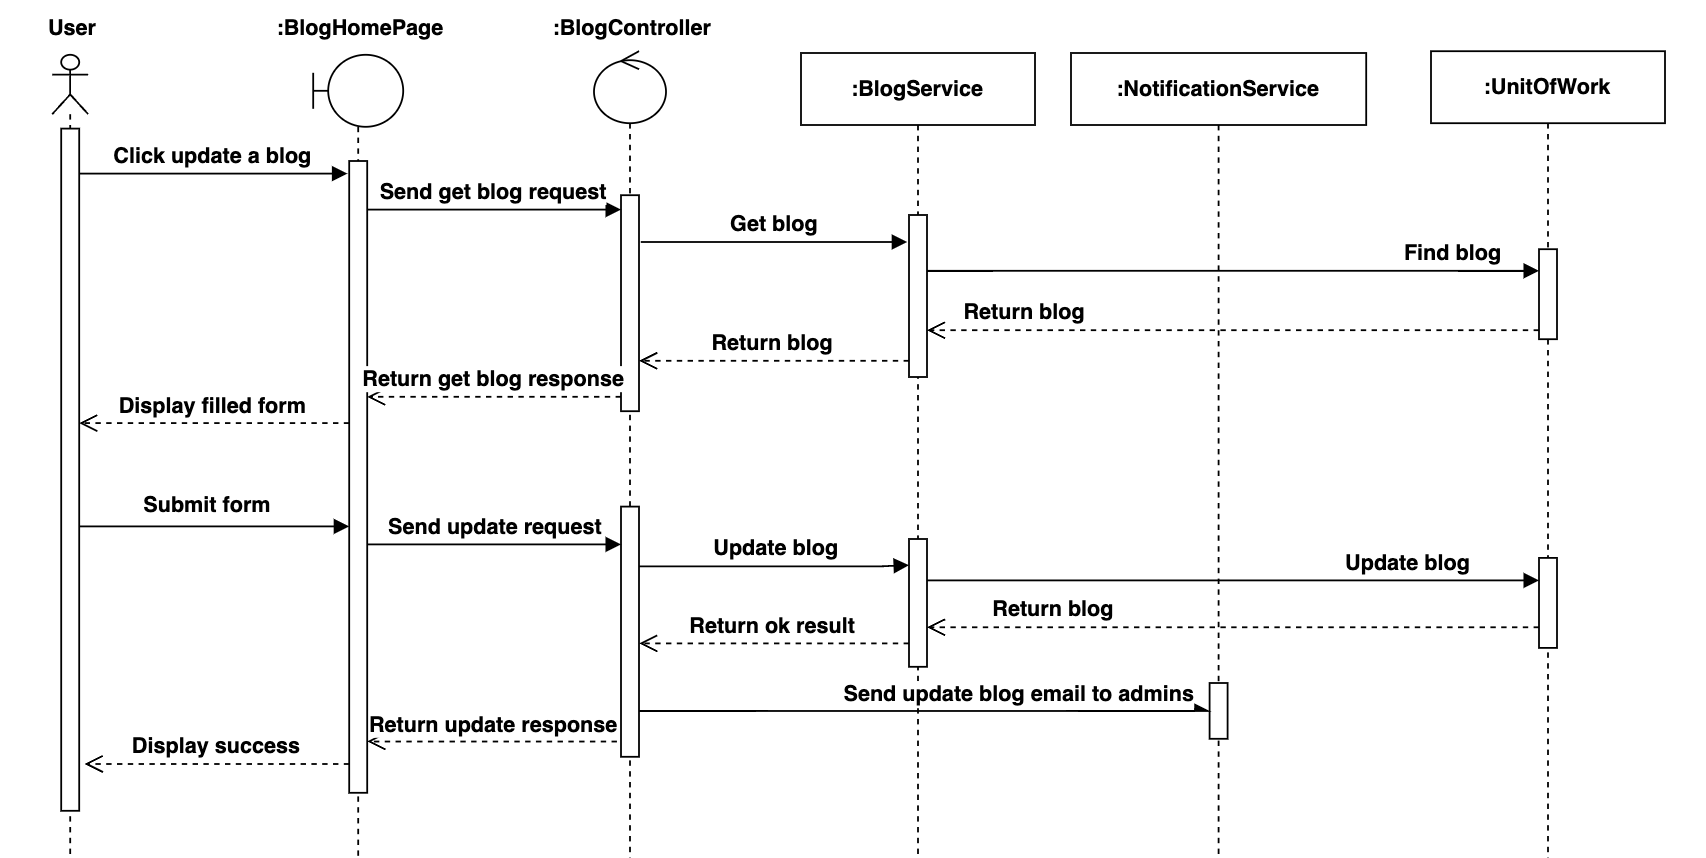
\includegraphics[width=0.9\textwidth]{Figures/update_blog_seq.png}
    \caption{Update blogs sequence diagram}
    \label{fig:update-blog-seq}
\end{figure}
\clearpage

\subsection{Access pets}
\begin{figure}[H]
    \centering
    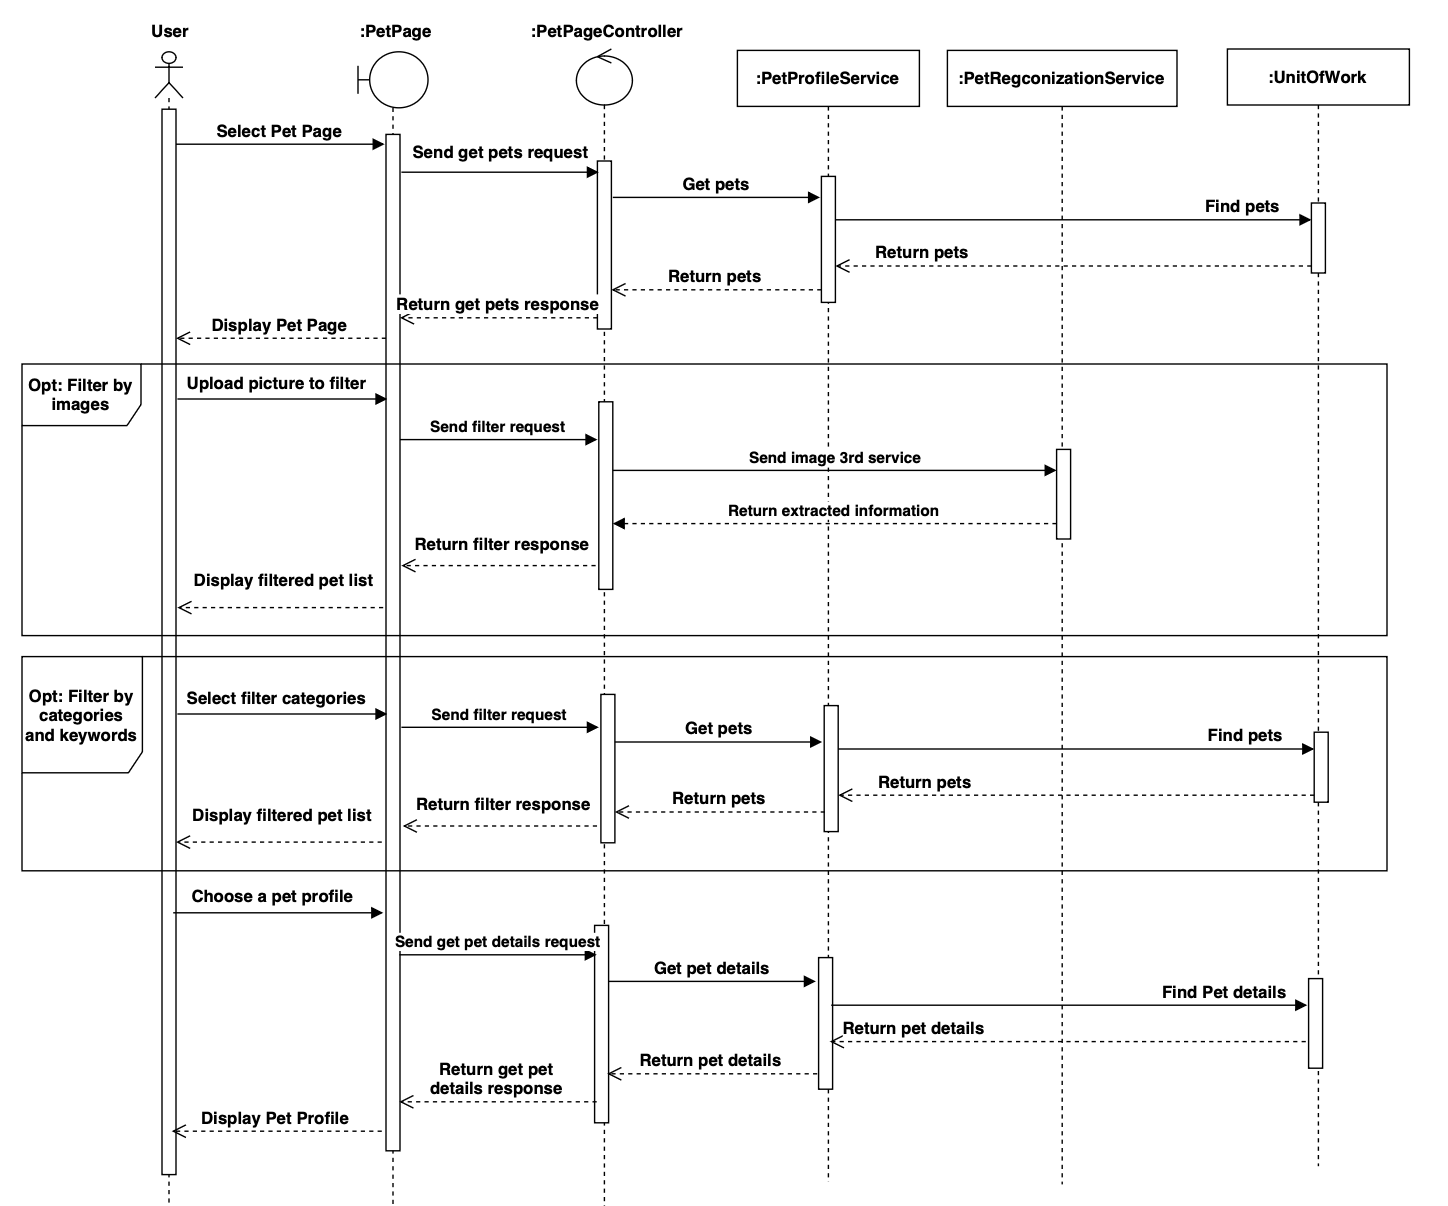
\includegraphics[width=0.9\textwidth]{Figures/access_pet_seq.png}
    \caption{Access pet sequence diagram}
    \label{fig:access-pet-seq}
\end{figure}

\subsection{Make payment}

\begin{figure}[H]
    \centering
    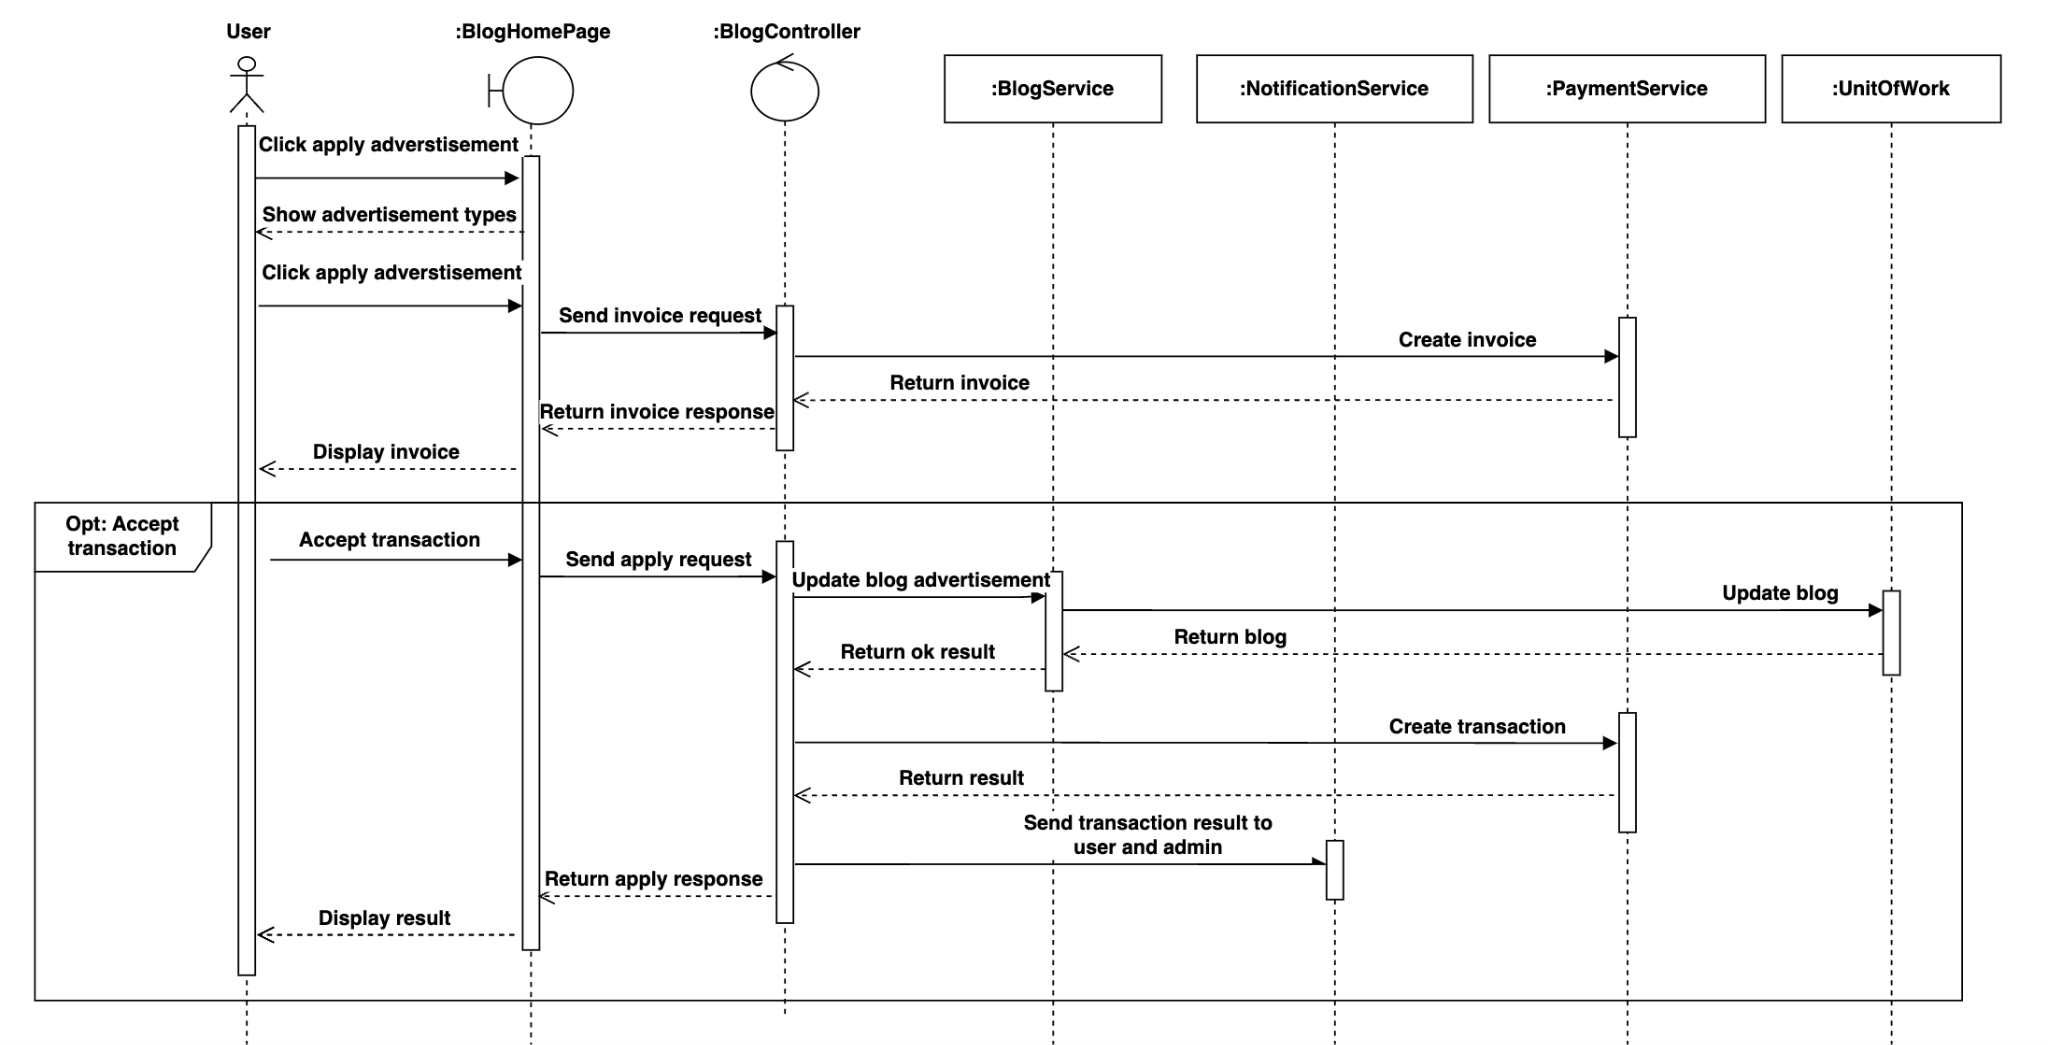
\includegraphics[width=0.9\textwidth]{Figures/payment_seq.png}
    \caption{Make payment sequence diagram}
    \label{fig:make-payment-seq}
\end{figure}


